\documentclass[12pt,a4paper]{article}
\usepackage[utf8]{}
\usepackage[T1]{fontenc}
\title{EP1200 - Datasys anteckningar}
\author{Yunshan Luo}


\renewcommand{\baselinestretch}{0.2}

\setlength{\hoffset}{-18pt}         
\setlength{\oddsidemargin}{0pt} % Marge gauche sur pages impaires
\setlength{\evensidemargin}{0pt} % Marge gauche sur pages paires
\setlength{\marginparwidth}{54pt} % Largeur de note dans la marge
\setlength{\textwidth}{481pt} % Largeur de la zone de texte (17cm)
\setlength{\voffset}{-18pt} % Bon pour DOS
\setlength{\marginparsep}{7pt} % Séparation de la marge
\setlength{\topmargin}{0pt} % Pas de marge en haut
\setlength{\headheight}{13pt} % Haut de page
\setlength{\headsep}{4pt} % Entre le haut de page et le texte
\setlength{\footskip}{27pt} % Bas de page + séparation
\setlength{\textheight}{720pt} % Hauteur de la zone de texte (25cm)

\usepackage{natbib}
\usepackage{graphicx}
\usepackage{amssymb}
\usepackage{amsmath} % Required for the align* environment
\usepackage{float}
\usepackage{pgfplots} 
\usepackage{algorithm}
\usepackage{mathrsfs}

\usepackage{algpseudocode} % test comment
\usepackage[hidelinks]{hyperref}
\pgfplotsset{compat=1.18}


\begin{document}
\title{DD2395 -- Computer security}
\maketitle
\newpage
\section{Lecture 1}
\subsection{Examination and grading}
\begin{itemize}
    \item LAB assignments: P/F bonus for the final grade at least 2 marks for A
    \item Exam: 100\% of the grade
\end{itemize}

\section{Lecture 2}
\subsection{Alice, Bob, Eve and Mallory}
\begin{itemize}
    \item Alice and Bob tries to send messages to each other
    \item Eve is an eavesdropper, she can read the messages
    \item Mallory is a malicious attacker, she can read and modify the messages
\end{itemize}

\subsection{Three goals fo cryptography}
\begin{itemize}
    \item \textbf{Confidentiality:} Messages cannot be read by anyone except the intended recipient
    \item \textbf{Integrity:} Messages cannot be modified wihtout being detected
    \item \textbf{Authentication:} I can prove that this message came from the person who claims to have sent it
\end{itemize}

\subsection{Keys}
\begin{itemize}
    \item \textbf{Symmetric key:} Alice and Bob both knows the value of the secret key
    \item \textbf{Assymmetric key:} A user has two keys, a secret key and a public key
    \item \textbf{Open design:} Everyone knows how the system is designed
\end{itemize}

\subsection{Confidentiality}
\begin{enumerate}
    \item Alice uses the key to \textbf{encrypt} the message
    \item Alice sends the encrypted message over the insecure channel
    \item Eve sees the encrypted message, but cannot read the original message
    \item Bob receives the encrypted message and uses the key to \textbf{decrypt} the message back into its original form 
\end{enumerate}
\begin{figure}[H]
    \centering
    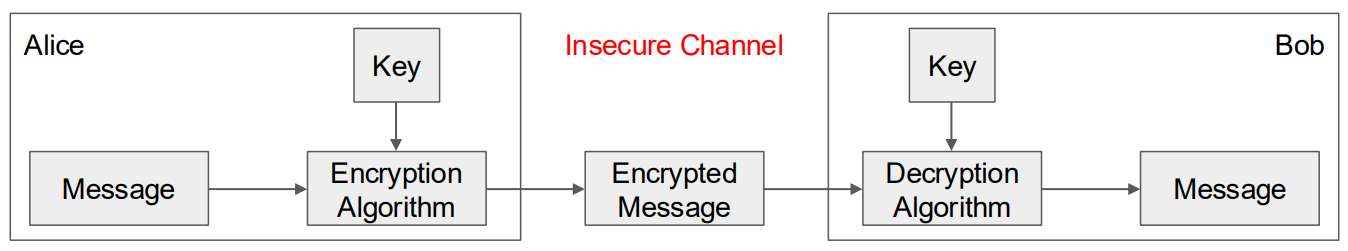
\includegraphics[width=0.9\textwidth]{Screenshot from 2026-08-31 14-06-04.png}
\end{figure}
\begin{itemize}
    \item \textbf{Plaintext: }The original message
    \item \textbf{Ciphertext: }The encrypted message
\end{itemize}

\subsection{Integrity and Authenticity}
Integrity and authenticity can be provided by using \textbf{tag} or signature on messages
\begin{itemize}
    \item Alice uses the key to generate a tag for the message
    \item Alice sends the message and the tag over the insecure channel
    \item If Mallory modifies the message, Bob will detect it when he checks the tag
    \item Bob receives the message and check if the tag is valid
\end{itemize}
\begin{figure}[H]
    \centering
    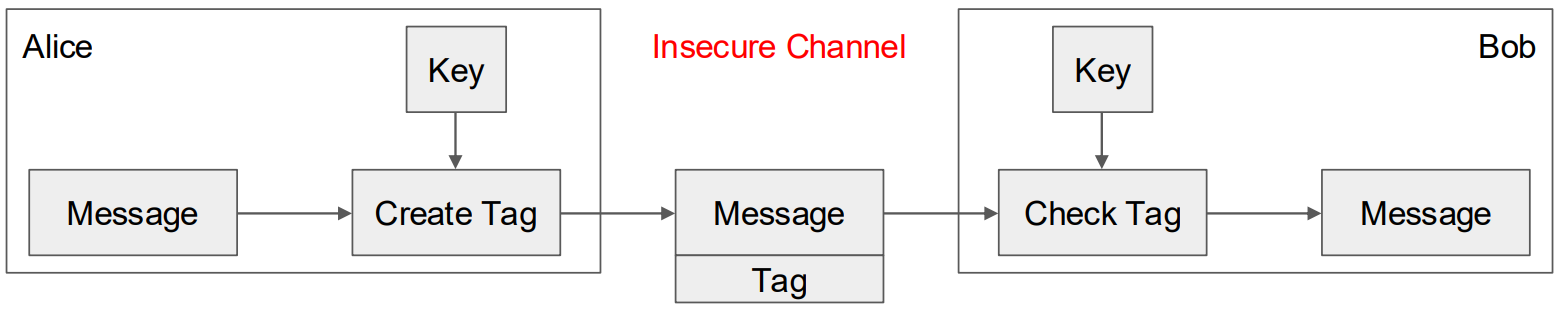
\includegraphics[width=0.9\textwidth]{Screenshot from 2026-08-31 14-19-35.png}
\end{figure}

\subsection{Threat models for confidentiality}
\begin{figure}[H]
    \centering
    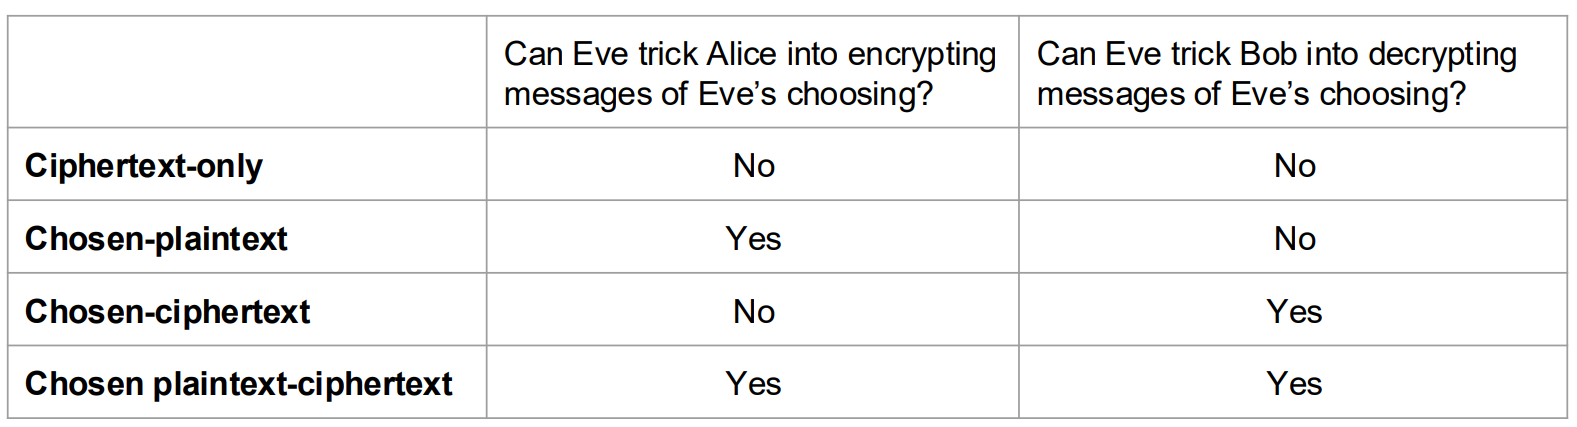
\includegraphics[width=1\textwidth]{Screenshot from 2026-08-31 14-23-36.png}
\end{figure}
\begin{itemize}
    \item The current lecture focuses on \textbf{Chosen-plaintext} 
\end{itemize}

\subsection{Cryptography Roadmap}
\begin{itemize}
    \item Symmetric-key
    \begin{itemize}
        \item Confidentiality:
        \begin{itemize}
            \item One-time pad
            \item Block ciphers (e.g. AES)
        \end{itemize}
        \item Integrity and authenticity:
        \begin{itemize}
            \item Hash functions
            \item MACs (e.g. HMAC) - Message Authentication Code
        \end{itemize}
    \end{itemize}
        \item Assymmetric-key
        \begin{itemize}
            \item Confidentiality:
            \begin{itemize}
                \item RSA encryption
                \item ElGamal encryption
            \end{itemize}
            \item Integrity and authenticity:
            \begin{itemize}
                \item Digital signatures (e.g. RSA, ECDSA)
            \end{itemize}
    \end{itemize}
\end{itemize}

\subsection{Symmetric Key Cryptography}
Alice and Bob shares a secret key. Symmetric cryptography has three algorithms:
\begin{enumerate}
    \item KeyGen() $\rightarrow$ Generates a key $K$
    \item Enc($K$, $M$) $\rightarrow$ Encrypts \textbf{plaintext} $M$ into \textbf{ciphertext} $C$
    \item Dec($K$, $C$) $\rightarrow$ Decrypts \textbf{ciphertext} $C$ using the key $K$
\end{enumerate}

\subsection{Confidentiality: IND-CPA definition}
\begin{enumerate}
    \item Eve may choose plaintext to send to Alice and receives their chiphertexts
    \item Eve issues a pair of plaintexts $M_0$ and $M_1$ to Alice
    \item Alice chooses either $M_0$ or $M_1$ encrypts it and do not tell Eve which one she chose
    \item Eve may again choose plaintext to send to Alice and receives their ciphertexts
    \item Eve guesses which plaintext Alice chose and wins if she guesses correctly
\end{enumerate}
An algorithm is \textbf{IND-CPA} secure if Eve cannot guess with probability larger than $50\% + \epsilon$. Where $\epsilon$ is a negligible advantage.

\subsection{Edge case: Length}
\begin{itemize}
    \item Cryptographic schemes are not allwed to leak the length of the message
    \item To prevent this there are two solutions:
    \begin{itemize}
        \item Make all messages the same length (unpractical)
        \item Pad messages to a fixed length (practical)
    \end{itemize}
\end{itemize}

\subsection{Negligible advantage}
For an encryption scheme with a k-bit key the advantage for Eve should be $\mathcal{O}(1/2^k)$.
\begin{itemize}
    \item $\epsilon = (\frac{1}{2})^{128}$ -- Currently unlikely
    \item $\epsilon = (\frac{1}{2})^{20}$ -- Fairly likely
    \item \textbf{Takeaway:} $\epsilon < (\frac{1}{2})^{80}$ is a current reasonable threshold
\end{itemize}

\subsection{One-Time pad key generation}
\noindent Encryption scheme
\begin{itemize}
    \item Given a random key $K$ of length $n$
    \item Given a message $M$ of length $n$
    \item $C = M \oplus K$ where $\oplus$ is the bitwise XOR operation
\end{itemize}

\noindent Decryption scheme
\begin{itemize}
    \item Given a random key $K$ of length $n$
    \item Given a ciphertext $C$ of length $n$
    \item $M = C \oplus K$ where $\oplus$ is the bitwise XOR operation
\end{itemize}

\subsection{One-Time pad functions}
\begin{itemize}
    \item \textbf{KeyGen()}
    \begin{itemize}
        \item Randomly generate an n-bit key $K$, where n is the length of your message
        \item We assume that Alice and Bob have a secure channel to share the key
        \item We generate a new key for every message
    \end{itemize}
    \item \textbf{Enc(K, M)}
    \begin{itemize}
        \item $M \oplus K = C$
    \end{itemize}
    \item \textbf{Dec(K, C)}
    \begin{itemize}
        \item $C \oplus K = M$
    \end{itemize}
\end{itemize}

\noindent One-Time pad is \textbf{perfectly secure} however not IND-CPA secure since the key can only be used once.

\section{Lecture 3}
\subsection{Block cipher}
\begin{itemize}
    \item An algorith that encrypts a fixed-size block of bits
    \item $E(K,M) = C$: Encryption
    \begin{itemize}
        \item Inputs: k-bit key $K$ and n-bit plaintext $M$
        \item Output: n-bit ciphertext $C$
        \item Written as $\{0,1\}^k \times \{0,1\}^n \rightarrow \{0,1\}^n$
    \end{itemize}
    \item $D(K,C) = M$: Decryption
    \begin{itemize}
        \item Inputs: k-bit key $K$ and n-bit ciphertext $C$
        \item Output: n-bit plaintext $M$
        \item Written as $\{0,1\}^k \times \{0,1\}^n \rightarrow \{0,1\}^n$
    \end{itemize}
    \item Properties of block ciphers
    \begin{itemize}
        \item $E_k$ is a permutation, $D_k$ is the inverse permutation
        \item Encryption and decryption is fast
        \item $E$ behaves like a random permutation
        \item $E(K,M)$ is always bijective 
    \end{itemize}
\end{itemize}

\subsection{Block cipher: Brute force attacks}
How hard is brute forcing a 128-bit key?
\begin{enumerate}
    \item We have to try $2^{128}$ keys
    \item $2^10 \approx 10^3$
    \begin{itemize}
        \item $2^{128} = (2^{10})^{12.8} \approx (10^3)^{13} = 10^{39}$ 
    \end{itemize}
    \item Supposed that we could try $10^{18}$ keys per second
    \item $10^{39} / 10^{18} = 10^{21}$ seconds $\approx$ 30 trillion years
\end{enumerate}
\newpage
\subsection{AES algorithm}
\begin{enumerate}
    \item Take plain text and shuffle it using the key
    \item Key sizes determines the rounds of shuffling
    \begin{itemize}
        \item 128-bit key: 10 rounds
        \item 192-bit key: 12 rounds
        \item 256-bit key: 14 rounds
    \end{itemize}
    \item Each round uses its own "round key" derived from the cipher key
    \item Each round consists of four operations:
    \begin{enumerate}
        \item \textbf{SubBytes()}: Each byte is replaced with a corresponding byte from a fixed table
        \item \textbf{ShiftRows()}: Each row of the state is shifted by a certain number of bytes
        \item \textbf{MixColumns()}: Each column of the state is multiplied by a fixed polynomial
        \item \textbf{AddRoundKey()}: Each byte of the state is XORed with a byte of the round key
    \end{enumerate}
\end{enumerate}
\begin{figure}[H]
    \centering
    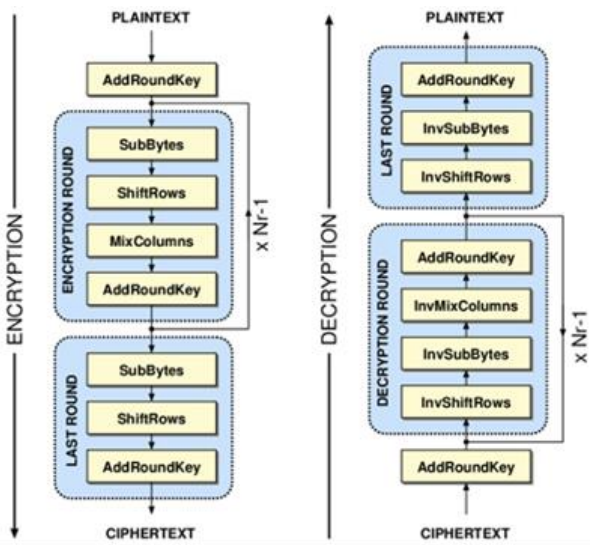
\includegraphics[width=0.65\textwidth]{AES.png}
\end{figure}

\subsection{IND-CPA analysis of block ciphers}
\begin{enumerate}
    \item Eve sends a pair of plaintexts $M_0$ and $M_1$ to Alice
    \item Eve receives the ciphertext $C$ of either $M_0$ or $M_1$ from Alice
    \item Eve requests the encryption of M0 again and receives the ciphertext $C_0$ from Alice
    \item \textbf{Strategy:} If $C = C_0$, then Eve guesses that Alice encrypted $M_0$, otherwise she guesses that Alice encrypted $M_1$
    \item Eve is guaranteed to guess correctly. Therefore not IND-CPA secure
\end{enumerate}

\subsection{Pros and cons of block ciphers}
\begin{itemize}
    \item Block ciphers are not IND-CPA secure
    \begin{itemize}
        \item The algorithm is \textbf{deterministic} because the same input always produces the same output
        \item A determinstic algorithm can never be IND-CPA secure because Eve can always guess correctly by sending the same plaintext twice
    \end{itemize}
    \item Block ciphers can only encrypt messages of a fixed size e.g. only 128 bits for AES
    \item Block ciphers uses XORs and bitshiting which is very fast and efficient
\end{itemize}

\subsection{Crypotgraphic Hashes}
Hash function $H(M)$ properies:
\begin{itemize}
    \item \textbf{Input:} Arbitrary length message $M$
    \item \textbf{Output:} Fixed length hash $h$
    \item \textbf{Deterministic:} The same input always produces the same output
    \item \textbf{Efficient:} The hash can be computed quickly
    \item \textbf{Security properties:} One way (preimage resistant), Collision resistance, random oracle
    \begin{itemize}
        \item \textbf{Random oracle:} There's no way to predict how changing the input will change the output
    \end{itemize}
\end{itemize}

\subsection{Preimage resistance}
\begin{itemize}
    \item \textbf{Informal definition:} Given an input $y$, it's infeasible to find any input $x$, such that $H(x) = y$
    \item \textbf{Formal definition: } $\forall A \in \mathcal{O}(n^k), \hspace{10pt} \Pr[A(H(x)) = y] < \epsilon, \hspace{10pt} \epsilon \approx 0$
\end{itemize}

\subsection{Collision resistance}
Collision is when two different inputs results in the same output
\begin{itemize}
    \item \textbf{Definition} $\forall x \neq x', \hspace{10pt} H(x) \neq H(x')$
    \item Hash functions ith no collisions are impossible due to the pigeonhole principle
    \begin{itemize}
        \item \textbf{Pigeonhole principle:} If you have more pigeons than pigeonholes, at least one pigeonhole must contain more than one pigeon
        \item In this case there are more possible inputs than outputs, so at least two inputs must map to the same output
    \end{itemize}
\end{itemize}

\subsection{Second preimage resistance}
\begin{itemize}
    \item \textbf{Definition:} Given an input $x$, it's infeasible to find another input $x' \neq x$, such that $H(x) = H(x')$
    \item Strong collision resistance $\implies$ Second preimage resistance
    \item \textbf{Collision resistance: } Attacker tries to find two inputs such that $H(x) = H(x')$
    \item \textbf{Second preimage resistance: } Attacker is any given an input $x$ and tries to find another input $x' \neq x$ such that $H(x) = H(x')$
    \item Broken second preimage resistance $\implies$ Broken collision resistance
\end{itemize}

\subsection{Length extension attacks}
\begin{itemize}
    \item \textbf{Length extension attack:} Given $H(x)$ and the length of $x$, but not x, an attacker can create $H(x || m)$ for any $m$ without knowing $x$
    \item SHA-1 and SHA-2 are vulnerable to length extension attacks
    \item SHA-3 is not vulnerable to length extension attacks
\end{itemize}

\subsection{Hashing and integrity}
\begin{itemize}
    \item Hashes themselves are unkeyed functions and don't provide integrity or authenticity
    \item Hashes can be used to build keyed functions that provide integrity and authenticity
\end{itemize}

\subsection{Message Authentication Codes (MACs)}















\end{document}